\chapter{chapter3}
\label{cha:Prüfstandsaufbau}


\section{Prüfstandsaufbau}
\label{sec:Prüfstandsaufbau}

Der Prüfstand besteht aus zwei Air Handling Units und einer Prüfbox, in der der Enthalpieübertrager installiert ist. Die Anordunung der Komponenten ist in \ref{fig:Technische Übersicht des Prüfstandes} dargestellt. 

Die Air Handling Unit 2 ist über einen DN 150 PVC-Schlauch mit der Prüfbox verbunden. So ist der Außenluftstrom zum Enthalpieübertrager übertragbar. Die Air Handling Unit 1 ist mit zwei PVC-Schläuchen mit der Prüfbox verbunden. So ist der Zuluftstrom vom Enthalpieübertrager zur Air Handling Unit 1 und der Abluftstrom von der Air Handling Unit 1 zum Enthalpieübertrager übertragbar. Ein vierter PVC-Schlauch führt den Fortluftstrom vom Enthalpieübertrager weg.
 

\begin{figure} [h]
	\centering
	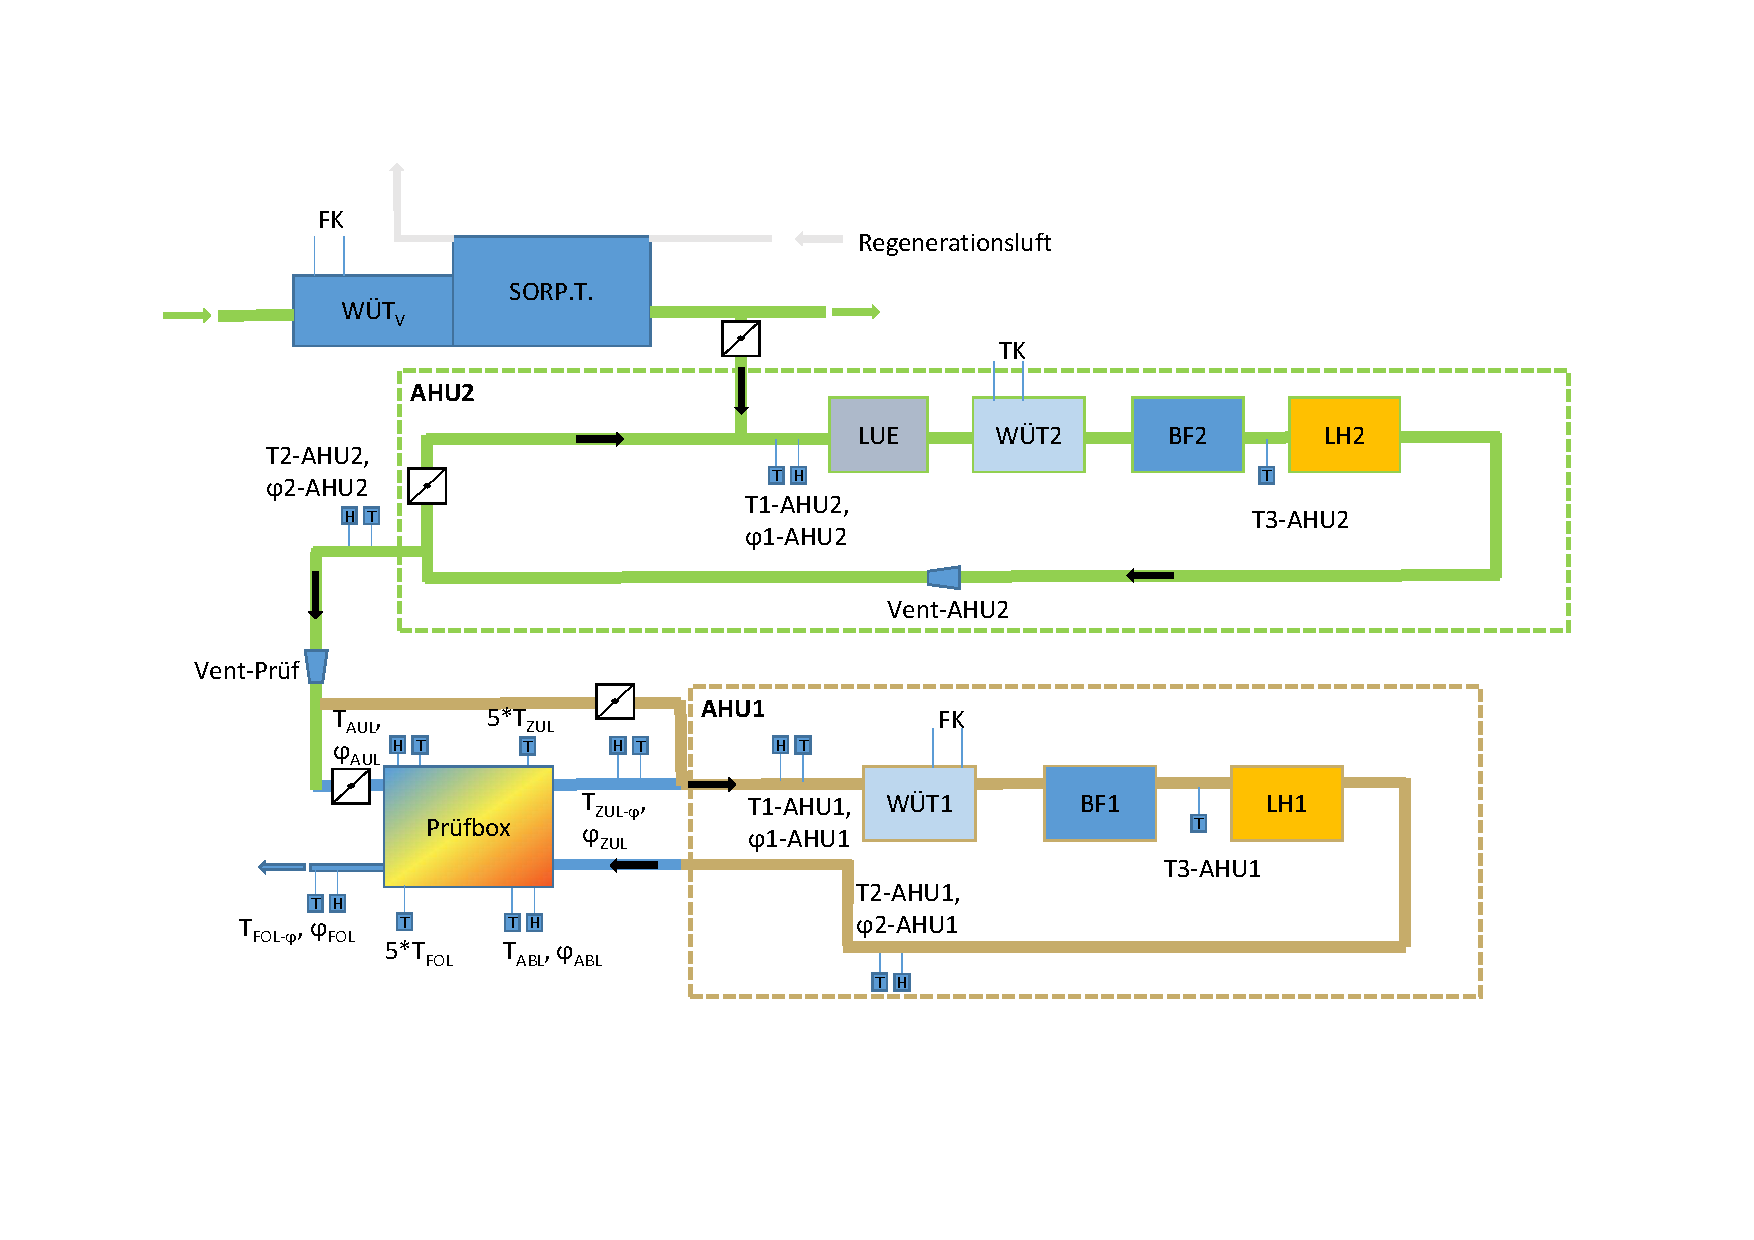
\includegraphics[width=0.98\textwidth]{pictures/Technische_Uebersicht_des_Pruefstandes.pdf}
	\caption{Technische Übersicht des Prüfstandes}
	\label{fig:Technische Übersicht des Prüfstandes}
\end{figure}

\subsection{Air Handling Units}
\label{Air Handling Units}

\subsubsection{Air Handling Unit 2}
\label{Air Handling Unit 2}

Die Air Handling Unit 2 simuliert die Umgebungsluft. Dazu weißt sie einen Sorptionstrockner $(SORP.T.)$ mit einer Vorkühleinheit $(WÜT_{V})$ und einem Ventilator auf, einen Lüfter $(LUE)$, einen 22 kW Wärmeübertrager $(WÜT2)$ zur Kühlung, einen elektrischen 6 kW Lufterhitzer $(LH2)$, sowie einen Dampfbefeuchter $(BF2)$. 

Um konstante Bedingungen für den Außenluftstrom zu gewährleisten ist in der Air Handling Unit 2 ein Luftstrom im Kreis förderbar. Hierbei können bis zu 4500 m³/h gefördert werden. 
Der Volumenstrom wird über ein Venturirohr $(Vent-AHU2)$ gemessen. Ein weiteres Venturirohr $(Vent-Prüf)$ misst den Außenluftstrom der zur Prüfbox fließt. Der Außenluftstrom beträgt maximal 450 m³/h. Die Regelung der Volumenströme erfolgt jeweils über Absperrklappen, die kontinuierlich verstellbar sind. 

Für die Temperaturregelung ist jeweils ein Temperatursensor Stromabwärts der Luftzufuhr $(T1-AHU2)$ und zu Beginn des Außenluftstroms verbaut. Außerdem befindet sich ein dritter Temperatursensor $(T3-AHU2)$ vor dem Lufterhitzer. Dies gewährleistet eine schnelle Reaktion der Regelung.

Zur Regelung des Dampfbefeuchters ist ein Feuchtesensor mit Temperaturfühler ($\varphi1$-AHU2)in der Außenluftleitung verbaut. Der Sorptionstrockner wird manuell gesteuert. Um notwendige Leistung des Sorptionstrockners zu ermitteln befindet sich ein Feuchtesensor inklusive Temperatursensor in der Leitung des Außenluftstroms $(\varphi2-AHU2)$.

Der Temperatursensor $T2_AHU2$ ist mit einen Temperaturwächter verbunden. Der Temperaturwächter reagiert bei 60 °C und trennt den Lufterhitzer von der Stromversorgung.
Der Wärmeübertrager wird auf der Primärseite von einem Solestrom $(TK)$ durchflossen. Zulaufseitig weist die Sole eine Temperatur von ca. -20 °C auf. Daher ist eine Abkühlung des Außenluftstromes auf Temperaturen von bis zu -10 °C möglich. 


\subsubsection{Air Handling Unit 1}
\label{Air Handling Unit 1}
 
Die Air Handling Unit 1 simuliert die Abluft. Sie weist einen elektrischen 4 kW Lufterhitzer (LH1), einen 3 kW Wärmeübertrager $(WÜT1)$ zum Kühlen und eine Dampfbefeuchter $(BF1)$ auf. Der Volumenstrom durch die Air Handling Unit 1 entspricht dem des Außenluftstromes. 

Zur Regelung der Luftbedingungen ist jeweils am Eintritt und am Austritt der Air Handling Unit 1 ein Feuchtesensor $(\varphi1-AHU1, \varphi2-AHU1)$ mit Temperaturfühler sowie je ein weiterer Temperatursensor $(T1-AHU1, T2-AHU2)$ verbaut. Außerdem ist ein Temperatursensor $(T3-AHU1)$ vor dem Lufterhitzer verbaut. 
Der Temperatursensor $T3-AHU1$ ermöglicht eine schnelle Reaktionszeit der Regelung. Der Temperatursensor $T2-AHU1$ ist außerdem mit einem Temperaturwächter verbunden, der bei 40°C auslöst. Der Temperaturwächter nimmt beim Auslösen den Lufterhitzer von der Stromversorgung.

Der Wärmeübertrager der Air Handling Unit 1 ist primärseitig an die Fernkälte $(FK)$ angeschlossen. Der Wasserstrom der Fernkälte besitzt eine Zulauftemperatur von ca. 8 bis 9 °C. Entsprechend ist es nicht möglich sehr kalte Temperaturen im Abluftstrom zu simulieren. Die minimale Temperatur der Abluft hängt von der Eintrittstemperatur der Luft und Leistung des Dampfbefeuchters in die Air Handling Unit 1 ab. Bei Temperaturen unter 10 bis 15 °C der Ablufttemperatur nimmt außerdem die Regeldauer stark zu. Die Temperaturdifferenz im Wärmeübertrager ist in diesem Fall so gering, dass nur eine geringe Leistung übertragen wird. Aufgrund des Wärmeübertragers tritt die Zuluft auch bei einem kalten Außenluftstrom zunächst mit erhöhter Temperatur in die Air Handling Unit 1 ein. Daher ist es während der Abkühlphase sinnvoll den Wärmeübertrager zunächst mittels eines Bypasses zu überbrücken. 


Alle in den Air Handling Units 1 und 2 verbauten Sensoren dienen der Regelung und Steuerung der Luftzustände. Alle zur Regelung verbauten Temperatursensoren entsprechen der Genauigkeitsklasse 1/3 Klasse B. Alle zur Regelung verbauten Feuchte-Sensoren weisen eine Genauigkeit von $\pm$ 1 \% relativer Feuchte auf.

\subsection{Prüfbox}
\label{Prüfbox}

Die Prüfbox dient als Halterung des Enthalpieübertragers und ermöglicht die Anströmung der Einlässe beziehungsweise die Abströmung an den Auslässen des Enthalpieübertragers. Abbildung \ref{fig:Aussenansicht montierte Prüfbox} zeigt die Prüfbox im montierten Zustand am Prüfstand. Von außen ist sie mit 22 mm Amaflex gedämmt, um die Temperaturverluste zu minimieren.

\begin{figure} [h]
	\centering
	\includegraphics[width=0.98\textwidth]{pictures/Aussenansicht_montierte_Pruefbox.jpg}
	\caption{Außenansicht montierte Prüfbox}
	\label{fig:Aussenansicht montierte Pruefbox}
\end{figure}

Um die einen hohe Reproduzierbarkeit der Versuche zu gewährleisten und die Übertragungsflächen im Enthalpieübertrager gleichmäßig zu nutzen, ist eine gleichmäßige Anströmung der Einlassflächen des Enthalpieübertragers notwendig. Die Norm … beschreibt Rahmenbedingungen unter denen Experimente mit Luftströmungen reproduzierbar durchgeführt werden können. Die Norm beschreibt für einen Rohrdurchmesser von  …. Eine Länge von … für die Einströmstrecke. 

Diese Bedingungen sind im Rahmen dieser Masterarbeit nicht Umsetzbar. Daher wurde eine Prüfbox konstruiert, die bei einer kurzen Einströmstrecke eine möglichst gleichmäßige Anströmung gewährleistet.

Abbildung \ref{fig:Prüfbox - Einlassseite Feedstrom} zeigt die Einlassseite des Feedstroms. Die Prüfbox ist auf der Einlassseite der Luftströme jeweils mit einem Lochblech versehen. Das Lochblech ist diagonal vor der Anströmfläche des Enthalpieübertragers angeordnet. Das Lochblech erzeugt einen Staudruck. Dies führt zu einer gleichmäßigeren Anströmung des Enthalpieübertragers. Der Luftzustrom in die Prüfbox verläuft orthogonal zur Anströmfläche des Enthalpieübertragers. Die diagonale Positionierung des Lochbleches gleicht den Druckverlust der Strömung entlang der Anströmfläche aus. So ermöglicht die Prüfbox eine gleichmäßige Anströmung des Enthalpieübertragers bei einer geringen Baulänge. Die die Homogenität der Luftströmung konnte im Rahmen dieser Masterarbeit nicht überprüft werden.

\begin{figure} [h]
	\centering
	\includegraphics[width=0.98\textwidth]{pictures/Pruefbox_Einlassseite_Feedstrom.jpg}
	\caption{Prüfbox - Einlassseite Feedstrom}
	\label{fig:Prüfbox - Einlassseite Feedstrom}
\end{figure}

% Norm anfügen

\subsection{Messsensoren}
\label{Messsensoren}

Im Gegensatz zu den in \ref{Air Handling Units} beschriebenen Sensoren, werden die Sensoren in Prüfbox sowie die Sensoren zwischen Prüfbox und den Air Handling Units als Messdaten für die Auswertung der Versuche genutzt. Die Lage der Sensoren ist so gewählt, dass sie möglichst genau den Zustand der Luft beim Eintritt in den Enthalpietauscher beziehungsweise beim Austritt aus dem Enthalpietauscher wiedergeben. Außerdem soll eine möglichst hohe Reproduzierbarkeit der Versuche gewährleistet sein.

\subsubsection{Verteilung der Sensoren}
\label{Verteilung der Sensoren}

Verteilung der Temperatursensoren
Für den Feed-Strom und den Sweep-Strom sind auf der Eingangsseite jeweils ein Temperatursensor $(T_{AUL}, T_{ABL})$ und ein Feuchtesensor $(PHI_AUL, PHI_ABL)$ in die Prüfbox verbaut. Der Temperatursensor wird mittels einer Messinghülse in Position gehalten. Feuchtesensor ist ebenfalls von außen an der Messinghülse befestigt. Der Abstand der beiden Sensoren beträgt so nur wenige Millimeter. Durch die kurze Distanz wird eine genaue Bestimmung des absoluten Feuchtegehalts der Luft $(x_{AUL}, x_{ABL})$ ermöglicht. 


\begin{figure} [h]
	\centering
	\includegraphics[width=0.98\textwidth]{pictures/Pruefbox_Auslassseite_Feedstrom.jpg}
	\caption{Prüfbox - Auslassseite Feedstrom}
	\label{fig:Prüfbox - Auslassseite Feedstrom}
\end{figure}

Abbildung \ref{fig:Prüfbox - Auslassseite Feedstrom} zeigt die Abströmseite des Feedstroms. Die Abströmseite des Sweepstrom ist identisch zu der des Feedstroms. Auf der Abströmseite beider Ströme sind an den Abströmflächen des Enthalpieübertragers jeweils fünf Temperatursensoren $(T_{ZUL-L}, T_{ZUL-Mitte}, T_{ZUL-R}, T_{ZUL-O}, T_{ZUL-U}, T_{FOL-L}, T_{FOL-Mitte}, T_{FOL-R}, T_{FOL-O}, T_{FOL-U})$ angebracht. Diese sind jeweils Kreuzförmig angebracht.

Durch die Kreuzstromgeometrie des Enthalpieübertragers entsteht ein Temperatur- und ein Feuchtegradient entlang der beta-Achse der Abströmfläche $(s.Kap...)$ . Auch eine inhomogene Strömung durch eine ungleichmäßige Anströmung oder Durchströmung des Enthalpieübertragers führt zu Temperatur- und Feuchtegradienten über der Abströmfläche. Dies ist in Kapitel \ref{Prüfbox} beschrieben. Die fünf Temperaturen jeder Seite werden zur Auswertung zu den Temperaturen $T_{ZUL}$ und $T_{FOL}$ gemittelt. Das vorgehen zur Mittelung ist in Kapitel ... beschrieben. 

Die Norm DIN... definiert die Messung der Temperatur in einem Luftstrom ...  Zur Messung der Temperatur wird ein Messpunktenetz aus … mal … Sensoren gefordert. Dies ist im Rahmen dieser Arbeit nicht möglich. Mit der gewählten Anordnung der Sensoren sind 3 Messpunkte je Koordinaten Richtung und Fläche möglich. Dies ermöglicht eine Ermittlung der Hauptwirkungen 2. Grades der beschriebenen Einflüsse. Eine Ermittelung der Wechselwirkungen ist auf diese Weise nicht möglich. 

An den Abströmseiten werden die Feuchtesensoren $(\varphi{_ZUL}, \varphi_{FOL})$ nicht in der Prüfbox positioniert. Es steht nur ein Sensor pro Seite zur Verfügung. Eine Messung kurz hinter der Abströmfläche des Enthalpieübertragers ist nicht sinnvoll. Dort weist der Luftstrom eine hohe Inhomogenität auf. Eine Messung an dieser Stelle kann zur Messung eines lokalen Feuchtewerts führen, der stark von dem Durchschnittswert im entsprechenden Luftstrom abweicht. Daher werden die Feuchtewerte erst nach einer Durchmischungsstecke gemessen. An dieser Stelle kann von einem thermodynamisch homogenen Strom ausgegangen werden. Zur Ermittlung der korrekten absoluten Feuchte $(x_{ZUL}, x_{FOL})$ wird an dieser Stelle die Temperatur $(T_{ZUL-\varphi}, T_{FOL-\varphi})$ erneut gemessen. 

Über die Durchmischungsstrecke ist absolute Feuchte konstant. Daher lässt sich mit den Temperaturen $T_ZUL$ und $T_FOL$ in der Prüfbox die relative Feuchte direkt nach dem Enthalpieübertrager errechnen.
Für alle beschriebenen Temperaturmessungen sind PT 100 Messsensoren der Genauigkeit 1/10 Klasse B nach DIN EN 60751 verbaut. Für alle beschriebenen Feuchtemessungen sind Honeywell HIH-Feuchtesensoren verbaut. Sie besitzen eine Genauigkeit von $\pm$ 3,5 \% relativer Feuchte. 

\section{Berechnung der Feuchte Werte}
\subsection{Berechnung der Absoluten Feuchte}
Die Berechnung der absoluten Feuchte erfolgt nach der Arden Buck Gleichung\cite{Buck.1981}. Danach ergibt sich die absolute Feuchte in g/kg für Temperaturen über 0 °C zu 

\begin{equation}
 x = \frac{18,015*f1_{wDP}{28,963*(P - f1_{wDP})}
\end{equation} 

wobei $f1_{wDP}$ der Dampfdruck ist und $P$ der Absolutdruck in hPa.
Der Dampfdruck berechnet sich zu

\begin{equation}
f1_{wDP} = \varphi*f1_{wT}/100
\end{equation}

wobei $f1_{wT}$ dem Sattdampfdruck bei der Temperatur $T$ entspricht und $\varphi$ die relative Feuchte angibt. $f1_{wT}$ berechnet sich nach Buck empirisch zu

\begin{equation}
f1_{wT} = EF_{w}*a_{w}*\exp((b_{w}-\frac{T}{d_{w}})*\frac{T}{T+c_{w}})
\end{equation}

wobei $a_{w}$\footnote{$a_{w}$ = 6,1121}, $b_{w}$\footnote{$b_{w}$ = 18,678}, $c_{w}$ \footnote{$c_{w}$ = 257,14} und $d_{w}$\footnote{$d_{w}$ = 234.5} empirische Werte für Werte sind, die die Sättigungsdampfkurve flüssigem Wasser beschreiben. $EF_{w}$ ist ein Fehlerkorrekturfaktor. Er korrigiert die veränderten Stoffeigenschaften von feuchter Luft gegenüber einem idealen Gas. Der Zusammenhang 

\begin{equation}
EF_{w} = 1 + 10^-4 * (7,2 + P * (0,0320 + 5,9*10^-6*T^2))
\end{equation}

für den Fehlerkorrekturfaktor ist ebenfalls empirisch ermittelt.

Für Temperaturen unterhalb von 0 °C ergeben sich auf Grund des Phasenübergangs von Wasser andere Stoffeigenschaften und somit andere empirische Zusammenhänge. 

Für die absolute Feuchte bei Temperaturen unter 0 °C bleibt der Zusammenhang entsprechend

\begin{equation}
 x = \frac{18,015*f1_{iDP}{28,963*(P - f1_{iDP})}
\end{equation}

wobei $f1_{iDP}$ den Dampfdruck bei Eis angibt. Der Dampfdruck von Eis ermittelt sich ebenfalls analog zu flüssigem Wasser zu

\begin{equation}
f1_{iDP} = \varphi*f1_{iT}/100
\end{equation}

wobei sich der Sättigungsdampfdruck f1_{iT} im Vergleich zu flüssigem Wasser ändert. Er ergibt sich für Eis zu


\begin{equation}
f1_{iT} = EF_{i}*a_{i}*\exp((b_{i}-\frac{T}{d_{i}})*\frac{T}{T+c_{i}})
\end{equation}

mit den Faktoren $a_{i}$\footnote{$a_{i}$ = 6,1115}, $b_{i}$\footnote{$b_{i}$ = 23,036}, $c_{i}$ \footnote{$c_{i}$ = 279,82} und $d_{i}$\footnote{$d_{i}$ = 333,7}. Die Regressionsfaktoren des Korrekturfaktors $EF_{i}$ ändern sich ebenfalls, sodass sich der Zusammenhang 

\begin{equation}
EF_{w} = 1 + 10^-4 * (2,2 + P * (0,0383 + 6,4*10^-6*T^2))
\end{equation}

ergibt. Die Gleichungen wurden aus den Zusammenhängen von \cite{.b} in Anlehnung an \cite{Buck.1981} entnommen. Sie weisen einen relativen Fehler von unter 0,5 \% auf.

\subsection{Berechnung der relativen Feuchte}
Die Rückrechnung zur relativen Feuchte erfolgt über den gleichen Zusammenhang. So ergibt sich die relative Feuchte zu

\begin{equation}
\varphi = \frac{f1_{wDP}*100}{f1_{wT}} 
\end{equation}

für flüssiges Wasser beziehungsweise zu 

\begin{equation}
\varphi = \frac{f1_{iDP}*100}{f1_{iT}} 
\end{equation}

für Eis. Der Dampfdruck lässt sich aus der absoluten Feuchte anhand der Gleichung

%\begin{equation}
%f1_{i,wDP} = \frac{P*x}{\frac{18,015}{28,963}+x} 
%\end{equation}

für flüssiges und festes Wasser ermitteln lässt.


Die Temperatur der konditionierten Luft lässt sich bis auf eine Genauigkeit von … einregeln. Die Feuchte der konditionierten Luft lässt sich bis auf eine Genauigkeit von… einregeln. Eine Aufzeichnung der gemessenen Temperaturen für die Sollwerte … findet sich in Abbildung.

